\documentclass[12pt]{article}
\usepackage{amssymb}
\usepackage{amsmath}
\usepackage{subfiles}
\usepackage[usenames,dvipsnames]{xcolor}
\usepackage{indentfirst}
\usepackage{microtype}
\usepackage{graphicx}
\usepackage{multicol}

\usepackage{xfrac}
\usepackage{relsize}

\usepackage{empheq}%braces

\usepackage{color}
\usepackage{fancybox}
\usepackage{marvosym}
\usepackage{tikz}
\usetikzlibrary{arrows}
\usepackage{geometry}
	\geometry{a4paper, total={170mm,257mm}, left=20mm, top=20mm, }

\renewcommand*\contentsname{Tartalomjegyzék}

\AddToHook{cmd/section/before}{\clearpage}

\newcommand{\niton}{\not\owns}

\begin{document}
\begin{titlepage}
	\centering \vfill
	{\textsc{Budapesti Műszaki és Gazdaságtudományi Egyetem} \par} \vspace{7cm}
	{\huge\bfseries Jelek és rendszerek 1\par} \vspace{0.5cm}
	{\large \textsc{Összefoglaló jegyzet}\par} \vspace{1.5cm}
	{\Large\itshape Készítette: Illyés Dávid\par} \vfill

	\noindent\fbox{%
    	\parbox{140mm}{
			\color{red}\textbf{Ez  a jegyzet nagyon hasonlóan van struktúrálva az előadás jegyzetekhez és fő célja, hogy olyan módon adja át a "A Programozás Alapjai 1" nevű tárgy anyagát, hogy az teljesen kezdők számára is könnyen megérthető és megtanulható legyen. }
   		}
	}

	\vfill {\large \today\par}
\end{titlepage}
\tableofcontents
\addtocontents{toc}{~\hfill\textbf{Oldal}\par}

    \section{1. előadás (2024.02.13.)}

        \subsection{Alapfogalmak}

            \begin{itemize}
                \item Jelek: Fizikai mennyiség, annka a matematikai leírása változó, ennek a számunkra fontos része a jel (pl: feszültség $u(t) = a(t) \sin \omega t$).
                
                    Jelek osztályozása \begin{itemize}
                        \item időfüggés
                        \begin{itemize}
                            \item[a,] folytonos idejű
                            \item[b,] diszkrét idejű
                        \end{itemize}
                    \end{itemize}
                \item Rendszer: Objektum modellje
                
                    $[y_1(t), \dots, y_m(t), ] = \scalebox{1.5}{y} \{[u_1(t), \dots, u_n(t)]\}$


                    Rendszerek osztályozása \begin{itemize}
                        \item Be- és kimenetek száma
                        \item Linearitás (lineáris/nem lineáris)
                        \item Kauzalitás (kauzális/akauzális)
                        \item Variáns/invariáns
                        \item Stabilis/labilis
                    \end{itemize}
                \item Hálózat
                    \begin{itemize}
                        \item Kirchhoff-hálózat
                        \item Jelfolyam hálózat
                    \end{itemize}
            \end{itemize}

        

	\section{2. előadás (2024.02.15.)}

        \begin{itemize}
            \item[a,] lineáris/nem lineáris
            \item[b,] rezisztív / dinamikus
            \item[c,] invariáns/variáns
                $u(t) = U\{i(t)\} \Rightarrow u(t-T) = U\{i(t-T)\}$

                pl.:$u(t) = R i(t) \rightarrow$

                    ha $R=const Rightarrow$ invariáns
                    ha $R=R(t) \Rightarrow$ variáns
            \item[d,] csatolt/csatolatlan
            
                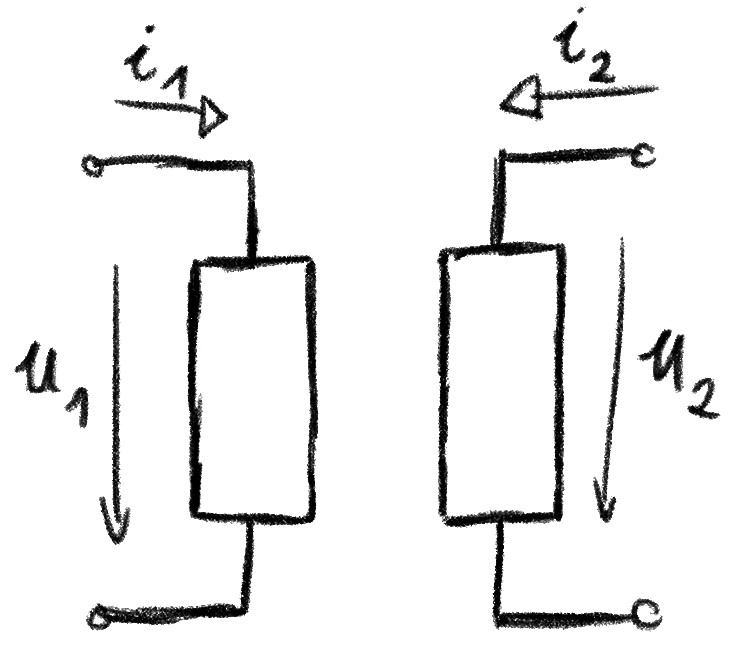
\includegraphics{img/1.png}

            \item[e,] passzív / aktív

            aktív - képes elektromos energiát termelni 
            passzív - csak fogyasztani képes
    
                Def: munkafüggvény 
    
                - $w(t) =\int_{-\infty}^{t}p(\tau)d\tau$
                A p a teljesítmény 
    
                $w(t) \geq 0 \Rightarrow $ passzív
            
                Def: lineáris, invariáns (LTI) 
    
                - Hálózat: lineáris invariáns kétpólusok és források összekapcsolásából áll
    
        \end{itemize}

         \subsection{speciális kétpólusok}

            1, feszültségforrás 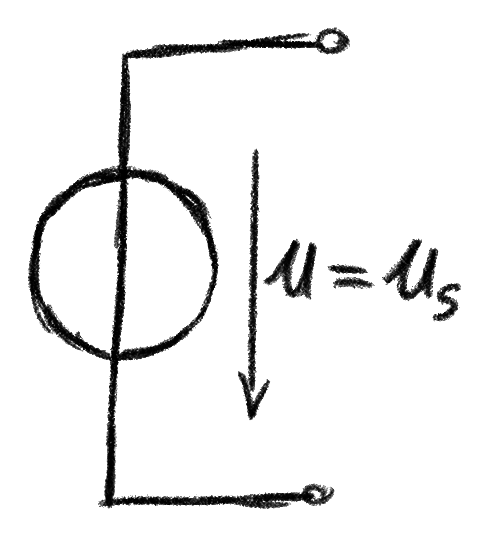
\includegraphics{img/2.png}

            2, speciális fesz. forrás (rövidzár) 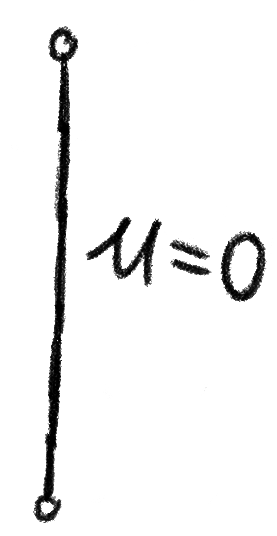
\includegraphics{img/3.png}

            3, áramforrás 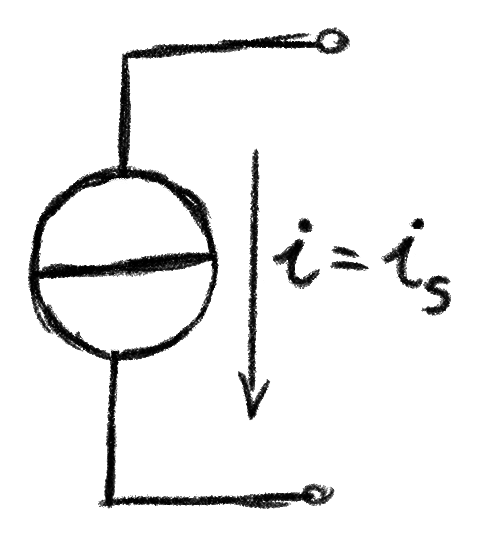
\includegraphics{img/4.png}

            4, szakadás 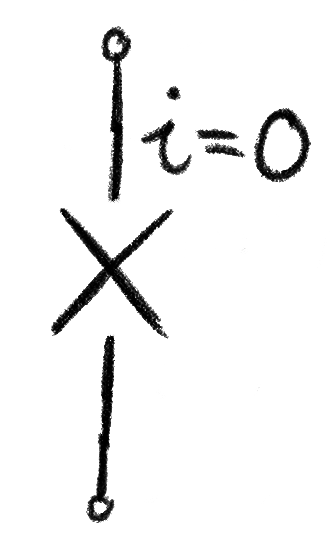
\includegraphics{img/5.png}

            5, lineáris, invariáns ellenállás 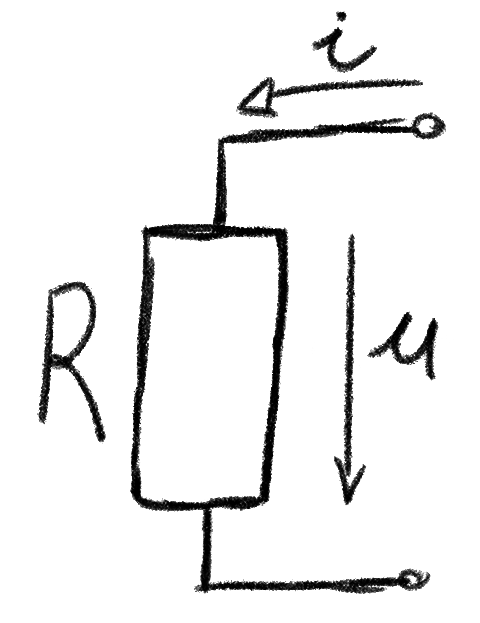
\includegraphics{img/6.png}

        \subsection{Kirchhoff törvények (1845)}

            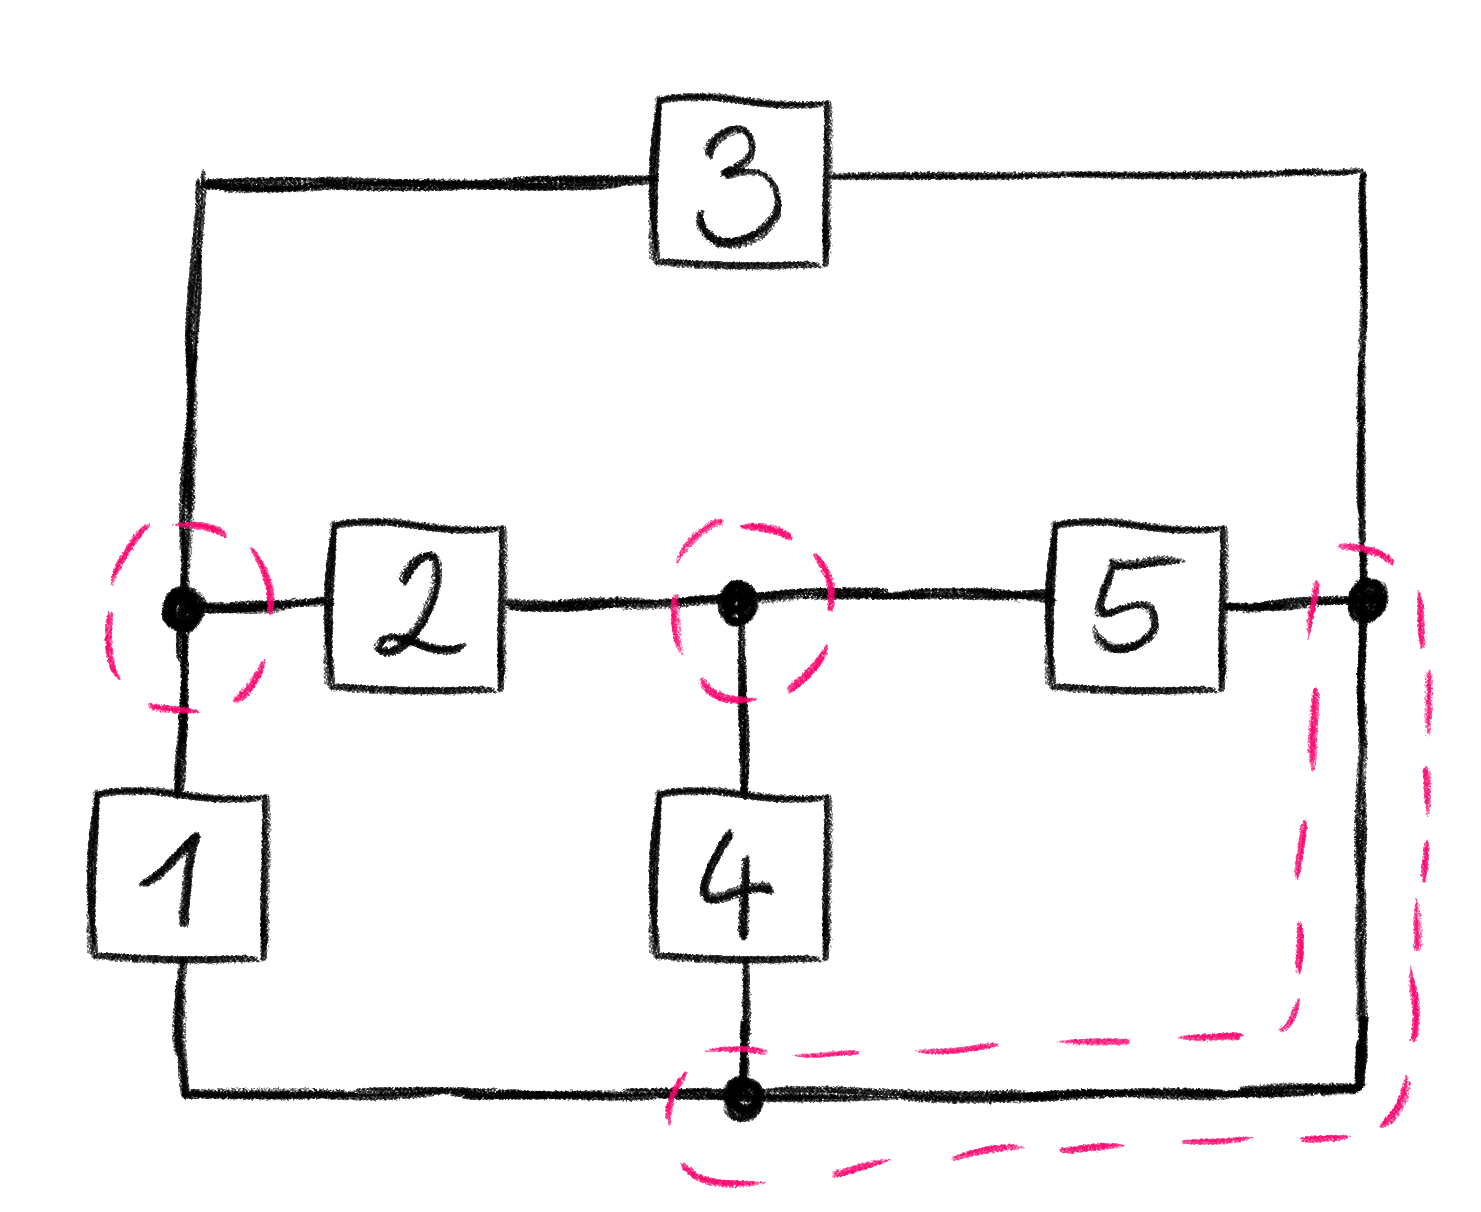
\includegraphics{img/7.png} 

            $b = 5$ kétpólus (branch)

            \textcolor{orange}{$n = 3$ csomópont (node)}

            \begin{itemize}
                \item[a,] Áramtörvény (ÁT) (töltésmegmaradás elve)
                 
                    $ \forall$ zárt felületre: \boxed{\sum_{k} i_k = 0}

                    $+ \rightarrow$ kifolyó áram

                    $- \rightarrow$ befolyó áram

                    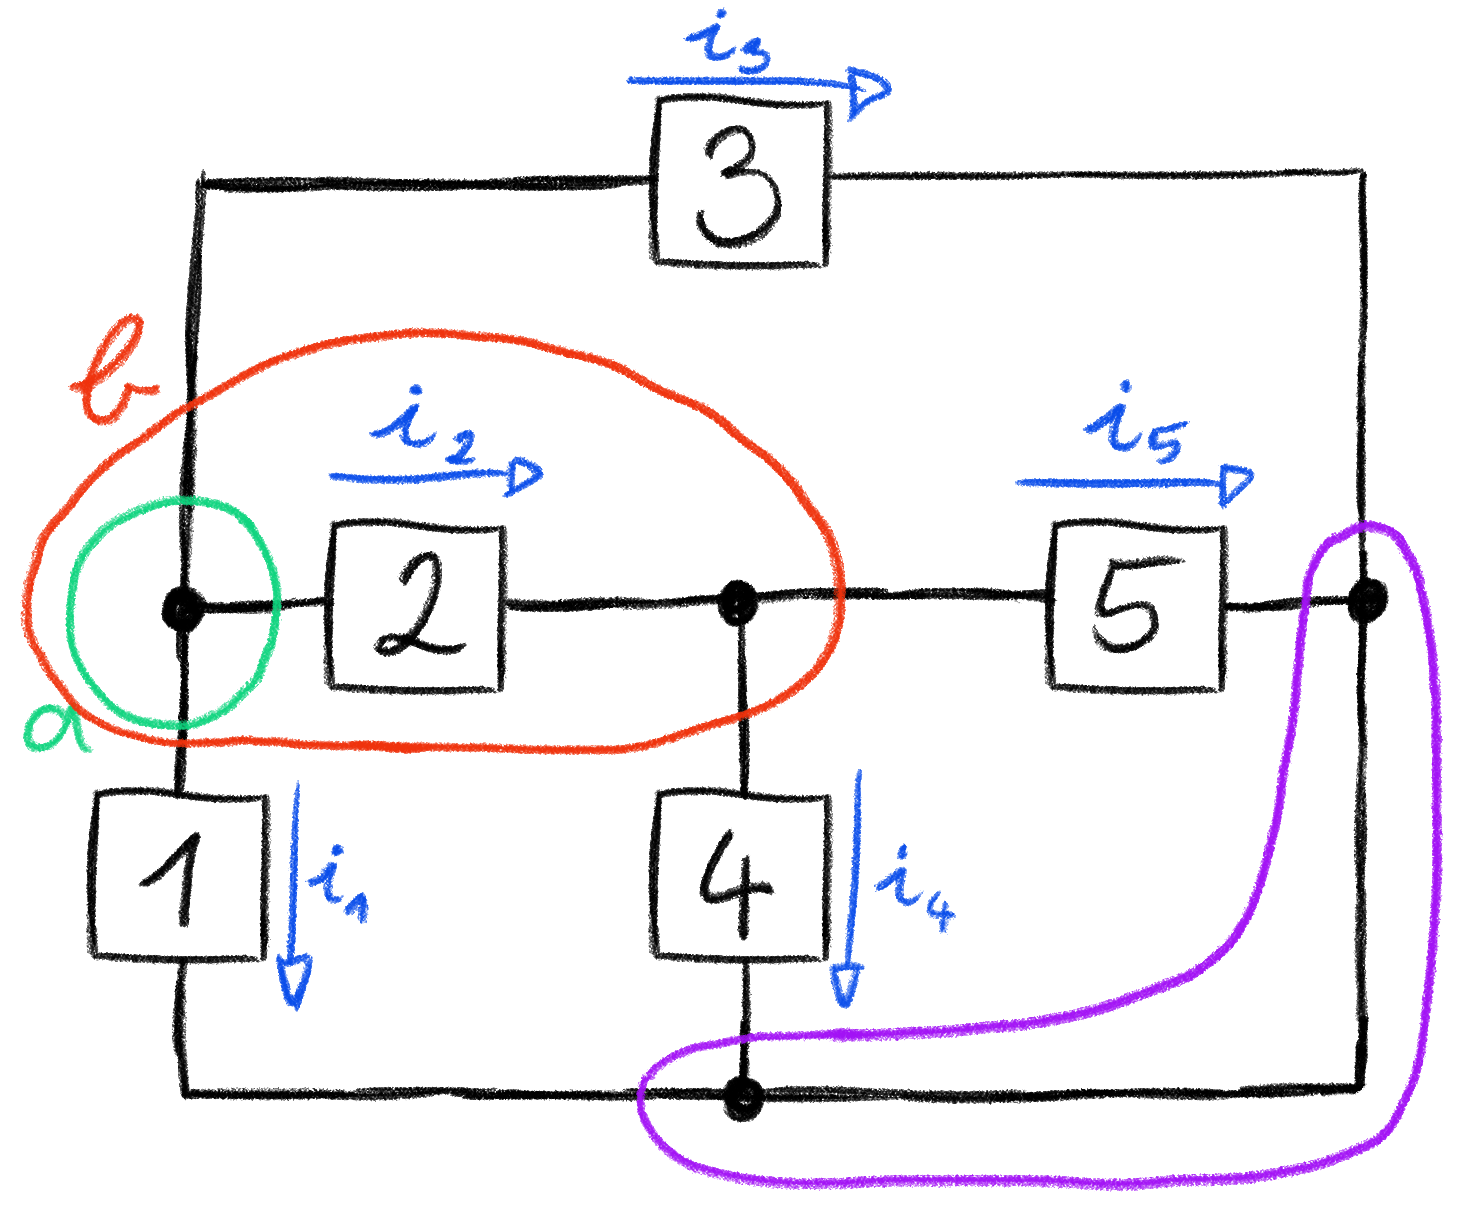
\includegraphics{img/8.png}

                    a: $0=i_1+i_2+i_3$

                    b: $0=i_1+i_4+i_5+i_3$
                    
                    c: $0=-i_3-i_5-i_4-i_1$

                    A $b$ és $c$ nem függetlenek egymástól.

                    A független áramtörvények max száma: $r=n-1$

                    Def: fundamentális áramtörvény rendszer:

                    \underline{Maximális} számú \underline{független} áramtörvény

                    Legegyszerűbb előállítás: egy kivételével az összes csomópontra felírunk egy áramtörvényt ($n-1$ számú csomóponti ÁT)

                    Pl: ,,a" és ,,c" 

                \item[b,] Feszültségtörvény (FT) (energiamegmaradás elve)
                
                    $\forall$ (irányított) hurokra \boxed{\sum_{k}i_k = 0}

                    + $\rightarrow$ hurok iránya

                    - $\rightarrow$ ellentétes irány

                    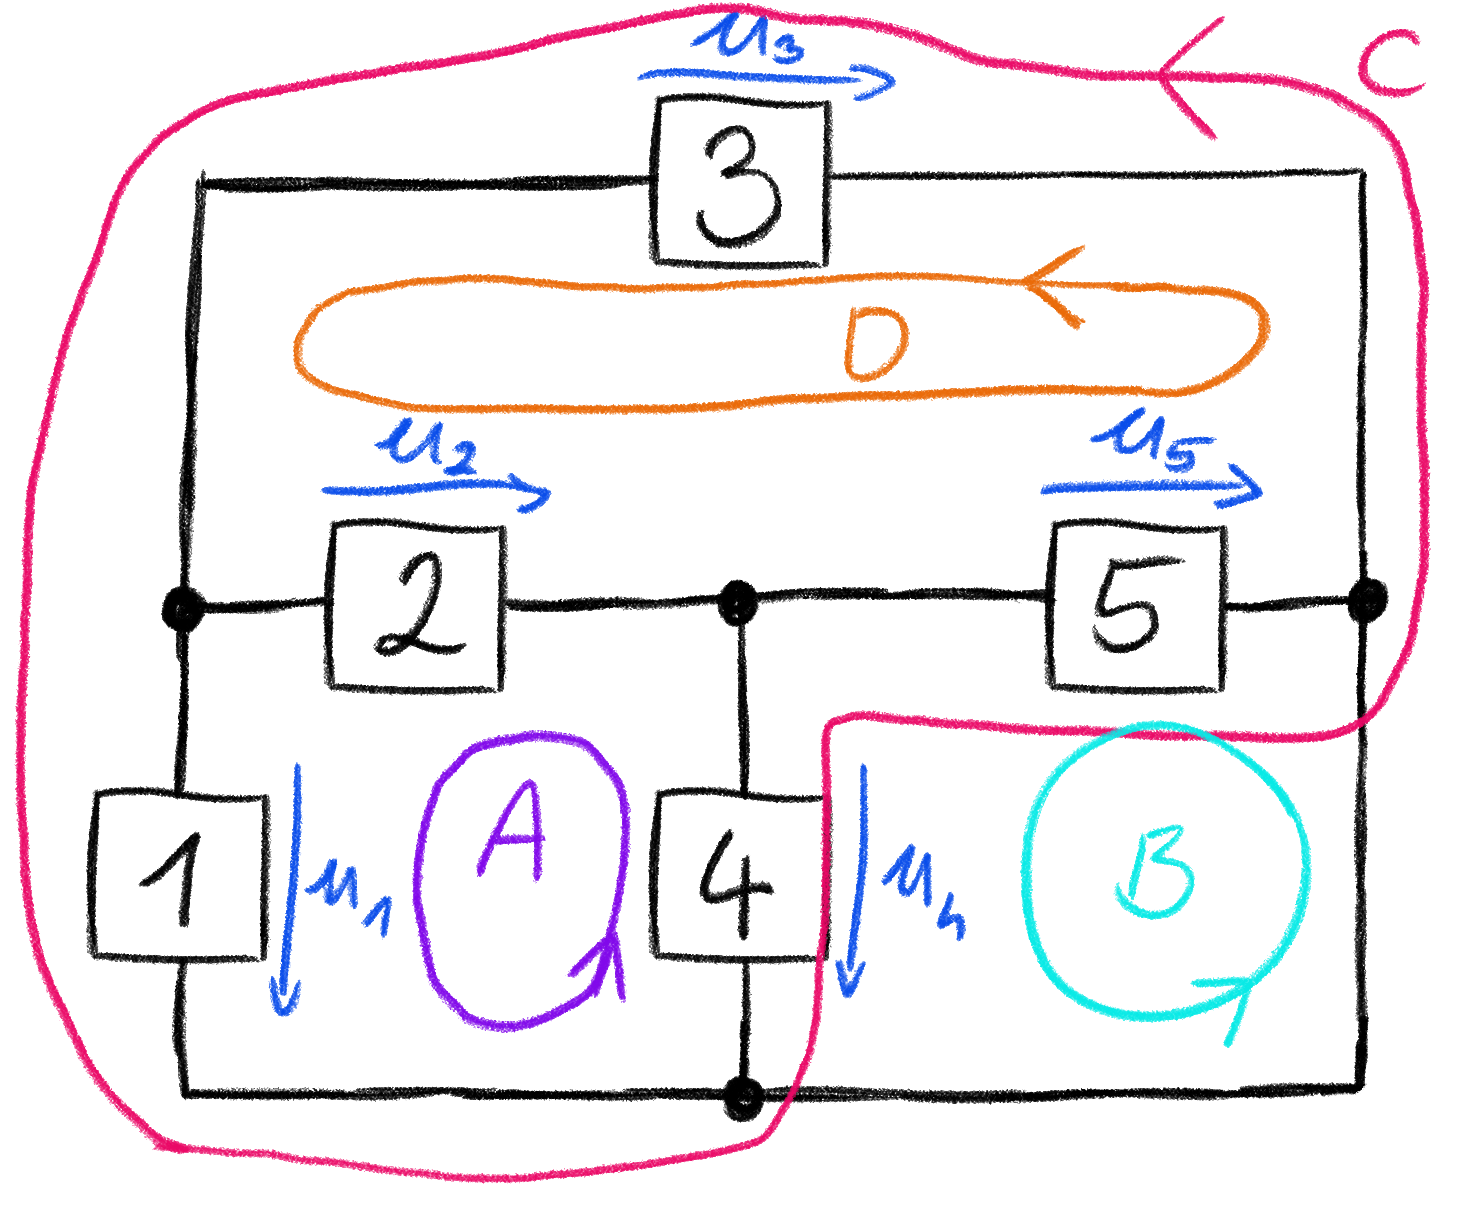
\includegraphics{img/9.png}

                    A: $0 = u_1-u_2-u_4$

                    B: $0 = u_4-u_5$

                    C: $0 = u_1-u_4+u_5-u_3$

                    D: $0 = u_2+u_5-u_3$

                    Ha a $C$-ből kivonjuk az $A$-t akkor a $D$-t kapjuk.

                    Független feszültségtörvények maximális száma: \boxed{$l = b - n + 1$}

                    Def: Fundamentális feszültségtörvény rendszer: max számú független feszültségtörvény.

                    Legegyszerűbb előállítás:

                    - hurkokat egymás után kell felvenni 

                    - $k$-dik hurok tartalmaz min egy kétpólust amelyet az \{$1, 2, 3, \dots, k-1$\} hurkok nem tartalmaznak

                    - vége: $k = l = b-n+1$

                \item[c,] Telegen-tétel

                    \boxed{\sum_{j=1}^{b}u_j'\cdot i_j'' = 0}

                    ' egyik eset 

                    '' másik eset 

                    a topológia mind két esetben ugyan az $\Rightarrow$ ' és '' ugyanaz az eset

                    $u_j i_j = p_j$: teljesítmény

                    \boxed{\sum_{j=1}^{b}p_j=0} energiamegmaradás elve

            \end{itemize}
    \subsection{A hálózat egyenletek teljes rendszere}

        $b$ kétpólus, n csomópont 

        $b$-feszültség és $b$ áram $\Rightarrow$ $2b$ változó

        felírható egyenletek: 
        \begin{itemize}
            \item $b$ karakterisztika
            \item $r=n-1$ Kirchhoff Áramtörvény
            \item $l=b-n+1$ Kirchhoff Feszültségtörvény
        \end{itemize}

        $\sum 2b$ egyenlet $\Rightarrow$ hálózat egyenletek teljes rendszere

        Def: reguláris hálózat: 

        HETR megoldható

        Megj: Lineáris hálózatban $\exists$ megoldás $\Rightarrow$ egyértelmű.

        Pl: \boxed{1} 

            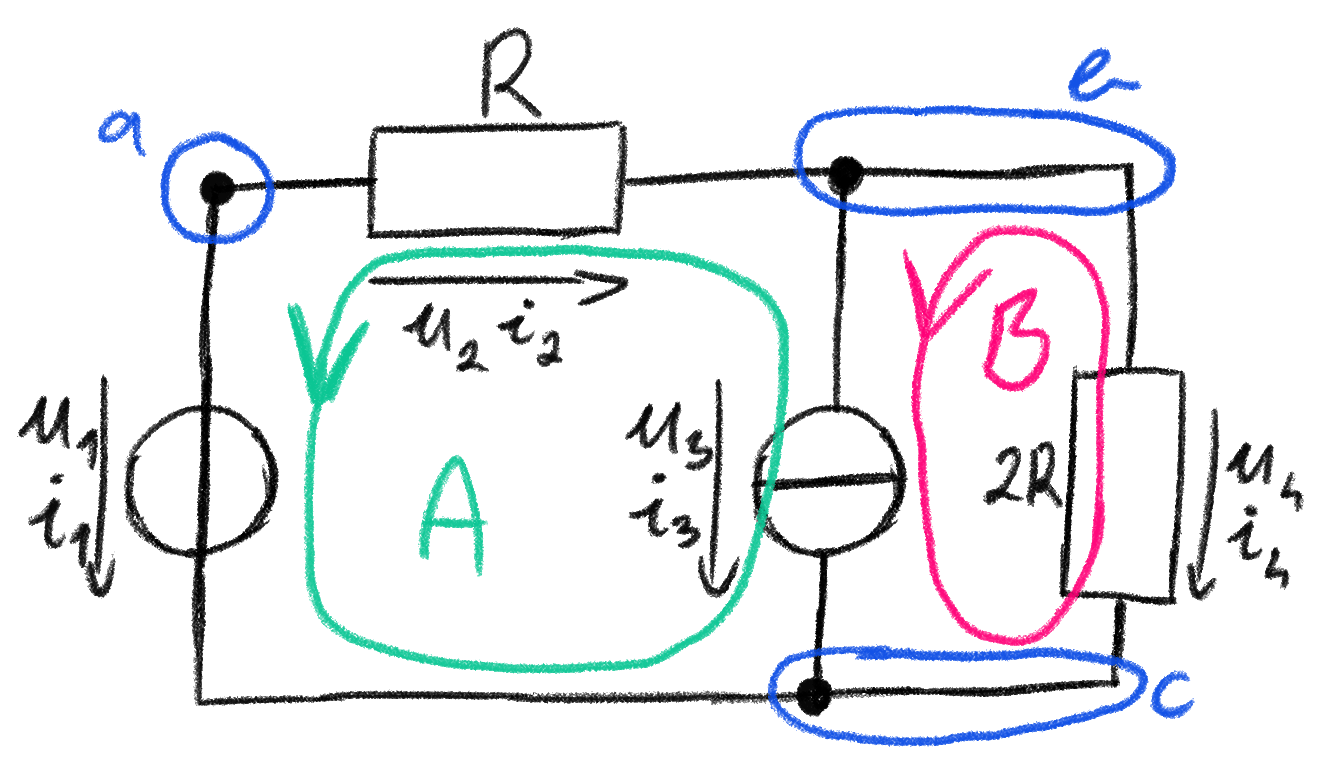
\includegraphics{img/10.png}

            $b = 4$

            $u_1 = u_s$

            $u_2=Ri_2$

            $i_3 = i_s$

            $u_4 = 2R i_4$

            (a fenti négy gecit jobb oldalról egy nagy kapocsal összehúzni)

            (ide kell egy vonal)

            a: $0=i_1+i_2$
            
            b: $0=i_3+i_4-i_2$

            (a fenti kettőt össze kapcsozni és utána írni hogy KÁT)

            A: $0=u_1-u_3-u_2$
            
            B: $0=u_3-u_4$ 

            (a fenti kettő gecit kapcsozni és utána KFT)

            ha $R \neq 0$ akkor az egyenletrendszer megoldható 

        Pl: \boxed{2}

            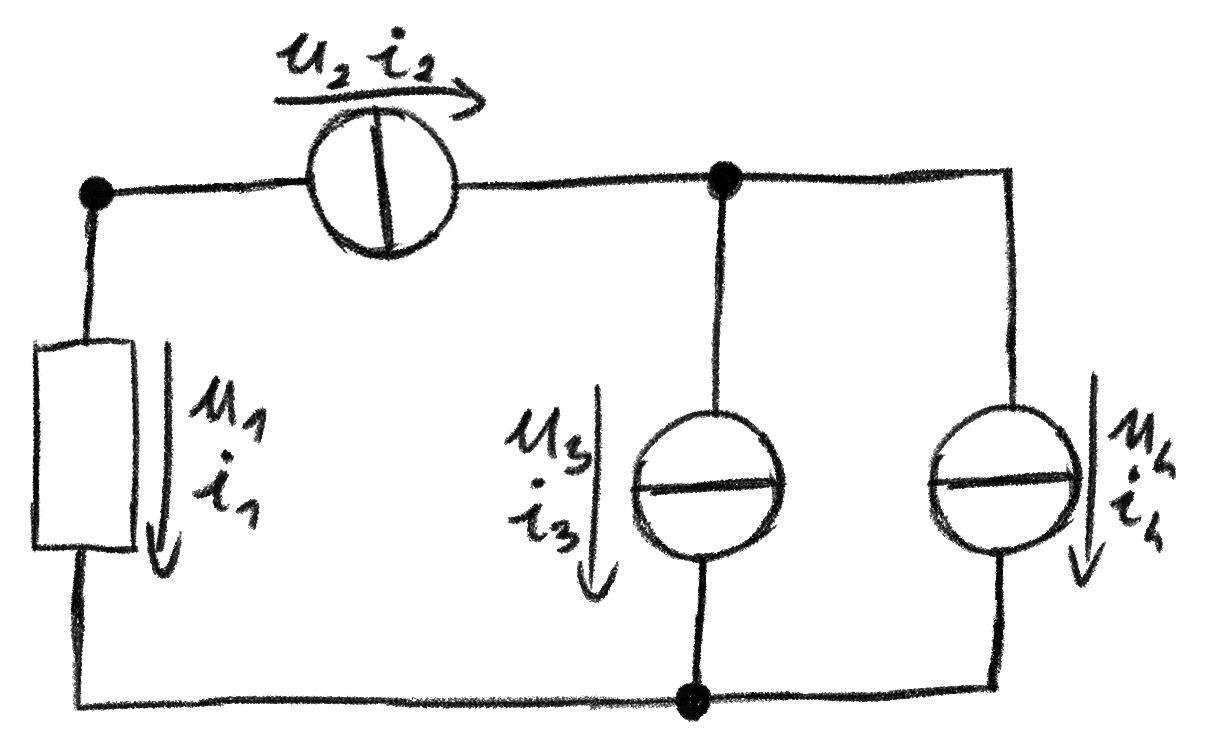
\includegraphics{img/11.png}

            karakterisztikák: 

            $u_1 = Ei_1$

            $i_2=i_{s,1}$
            
            $i_3= i_{s,2}$
            
            $i_4=i_{s,4}$

            b: $0=-i_2+i_3+i_4$

            \Lightning \;nem reguláris hálózat

        
\end{document}


\begin{subequations}
    \begin{empheq}[right={\empheqrbrace =f(x)}]{align}
        v =& v_0 + at \tag{1-11} \label{1-11}\\
        v =& x_0 + v_0t+\frac{1}{2}at^2 \tag{1-12} \label{1-12}\\
        v_2 =& v_0^2+2a(x-x_0) \tag{1-13} \label{1-13}
    \end{empheq}
  \end{subequations}